\documentclass[a4paper,10pt]{article}
\usepackage[utf8]{inputenc}
\usepackage{authblk}
\usepackage{tabularx}
\usepackage{url}
\usepackage{graphicx}
\graphicspath{{images/}}
\usepackage{caption}
\usepackage{subcaption}

\title{SuperMat: Construction of a linked annotated dataset from superconductors-related literature}
% \title{SuperMat: Construction of a linked annotated dataset for superconductors material discovery}
% \title{SuperMat: Construction of a linked annotated dataset to support superconductors material research}

\author[1]{Luca Foppiano\thanks{FOPPIANO.Luca@nims.go.jp}}
\author[1]{Sae Dieb}
\author[1]{Akira Suzuki}
\author[2]{Pedro Baptista de Castro}
\author[2]{Suguru Iwasaki}
\author[2]{Yan Meng}
\author[2]{Terashima Kensei}
\author[2]{Yoshihiko Takano}
\author[1]{Masashi Ishii\thanks{ISHII.Masashi@nims.go.jp}}

\affil[1]{Material Database Group, MaDIS, NIMS, Japan}
\affil[2]{Nano Frontier Superconducting Materials Group, MANA, NIMS}

\begin{document}

\maketitle

\begin{abstract}
% background and related work 
% material science 
% our work 

%The creation of large collaborative projects such as the Materials Genome Initiative~\cite{material_genome_initiative}, contributed to accelerate the change, however the amount of structured data represent a negligible part of the potentially available information.

%At the moment, the only available database for superconducting material discovery is Supercon, which is old, small (only 30000 entries) and outdated. There is needs of modernising or rebuilding the current manual process, which cannot keep-up with the current publication rate. 
% We are currently working on a collaborative project to implement a system for mining information from superconductors-related literature using different approaches of machine learning and rule-based. 

% We annotated entities such as materials, classes, measurement methods, and properties such as superconducting critical temperature values and expressions, and critical pressure. We linked materials with critical temperature, pressures, and measurement methods. 


% importance of text and data mining in material research (max 2 sentences) 
In materials science, abundant publications are available as knowledge source. However, information are presented mainly as text, which cannot be used as machine-readable media.
% information provided as text in a non-standardised and unstructured form, is 
The development of Text and data mining (TDM) processes is necessary to exploit this prosperity of information and scientists can benefit from this information overloading, for example, by semantic information retrieval, or by automatic document synthesis. 
In material discovery, breakthrough can be achieved by providing potential candidate materials in respect of certain properties, for example superconductivity or magnetic capabilities. 
%to accelerate toward breakthrough by exploiting the vast knowledge hidden in scientific literature. 

% The National Institute for Materials Science (NIMS) has been investing in establishing TDM processes to support material discovery. 
% manually constructing several databases to support materials research, and SuperCon\footnote{\url{http://supercon.nims.go.jp}} was a hopeful data source for superconductor domain. 
% Importance of superconducting material research 
Superconductors materials are already used as components in many applications~\cite{Hoshino2015InnovativeLR, Kizu2010ConstructionOT, Cardani2017NewAO, THOMAS201659}, and the research is still active~\cite{Drozdov_2019} but requires effort to fully switch to a data-driven approach\cite{Hamlin2019SuperconductivityNR}. 

% other attempts 
% However, only few attempts of applying TDM in materials literature have been described by \cite{Dieb2011ConstructionOT}, \cite{court2018auto} and \cite{kononova_text-mined_2019}. 

%% What we did 
We created a new dataset to provide solid foundations for establishing TDM processes for researchers of the superconductors domain and beyond: SuperMat (Superconductor Materials). Supermat is an annotated dataset of linked data of materials, properties and conditions from scientific literature. 

% How we did it 
This work has been carried out as collaborative project between computers and materials scientists and includes the documentation of the process and the annotation guidelines.
Our work is articulated over an iterative process composed by 4 main tasks: (1) relevant information selection, (2) tag-set and relationship design, (3) annotation rules definitions, and (4) validation by domain experts.
The dataset, composed by 114 articles and 9966 entities  (or which, 4000 unique), contains annotations of materials, samples, classes, properties (superconducting critical temperature, measurement method), and conditions (applied pressure). 
Relationships between certain entities is also annotated:  superconducting critical temperature (\textit{Tc}) with parametric conditions such as pressure values, and the used methods of measurements, when specified.

% What we found out 
We measured the Inter Annotation Agreement (IAA) between different classes of technicians (Computer Scientist, Material Scientists and Graduated Students) compared with domain experts. We reached a satisfying average agreement with domain experts. We noticed that students of materials science were challenged the most, indicating that the knowledge of only physics is not enough to successfully carry out the annotation task.

% What we conclude
SuperMat can be used to develop TDM processes for many complementary tasks such as information retrieval, document synthesis, information clustering. 
Our methodology and guidelines provides a trail that can be followed as a general approach in other domains. 
We utilised this dataset to train a sequence labelling system, which was then applied to semantically enhance a search engine for scientific documents and a document classification system using superconductors-related classes. 
\end{abstract}

\newpage

\section{Background and summary}
% Introduction, why text is important for scientific knowledge? 
The vast majority of scientific knowledge is available, with overwhelming abundance~\cite{Grigas2017JustGI, Khabsa2014TheNO, OrduaMalea2015MethodsFE, Bjrk2009ScientificJP} through published papers and articles. 
However, most of the information are presented as text, which is an arbitrary and unstructured form of communication, difficult to be used as machine readable media. 
% TDM and its importance - next sentence needs to link the a) abundance, and b) unstructured with the end result (structured data) -> TDM For the win... 

The computer-assisted process for identifying and collecting information from scientific literature, also referred to as Text and Data Mining (TDM), is a supportive asset for scientific research. 
In the past decades, TDM processes have evolved their ability to perform automatic document processing such as document synthesis, information retrieval and entity extraction. 

%The establishment of Text and Data Mining (TDM) processes is an unavoidable step to bridge information collected from scientific literature toward data-driven discovery. 

Looking at the scientific literature, several corpora has been created in other domains, to mention the most important: BioCreative IV CHEMDNER corpus~\cite{Krallinger2015TheCC} in chemistry, and Genia~\cite{Kim2003GENIAC} and GENETAG~\cite{Tanabe2005GENETAGAT, Ohta2009IncorporatingGA} in biology. In material science, we can mention NATDEV~\cite{Dieb2016} to support research of nanocrystal devices and, a material-synthesis corpus, for extracting systhesis recipes~\cite{kononova_text-mined_2019}. 

% Practical example in biology 
In biology, TDM has been applied in information extraction to identify agents interaction (e.g. bacteria, virus, genes, proteins)~\cite{10.1371/journal.pone.0004554, Krallinger2010, Krallinger2009ExtractionOH} or to support the research against serious diseases, like cancer~\cite{Krasnitz2019CancerB}. 
Chemical compounds name disambiguation, synthesis extraction and retrieval are other examples of TDM applications in chemistry~\cite{Hawizy2011ChemicalTaggerAT}.

% Dieb: Why collecting information from text is useful for material science? 
Materials science has been lagging behind. In many areas, materials scientists relies on theoretical approaches, such as Density Functional Theory (DFT) or ab-initio calculations, often based on manually extracted data. 
The adoption of data-driven computation (today called Materials Informatics (MI)) had been facing several challenges: lack of data standard, difficult to understanding the practical data-driven applicability, wide variety of conflicting stack-holders, and missing incentives to contributed to large collaborative initiatives~\cite{Hill2016MaterialsSW}. 

%% Add a sentence that state how TDM processes can help research in material science 
Like in other disciplines, materials scientists can benefit from TDM processes in many ways. 
For example, reducing the time needed looking for information by providing semantically enriched search engines able to accept very precise query~\cite{Liu2019SurfaceMR}. 
Secondly, and equally important, is to ease off the burden to collect structured data. Automatic process for dataset extraction will enable scientists to focus and leverage computing power for finding deeper relationships between information potentially unrelated.
All these process cannot be easily established without basic resources like dictionaries, lexicons, datasets. Materials-related or physical quantities dictionaries or publication-based datasets with annotated entities to mention some examples. 

%For example, to help researchers retrieving information based on very granular search queries, to extract structured datasets automatically, or to aggregate information by semantic similarity. suitable to be the input data of deep analysis processes   or properties prediction (curie temperature, magnetocaloric temperature, etc...).

% Superconductors domain
%   - concrete example of superconducting case -> which properties or information can be useful for superconducting material scientists? [Suzuki/Terashima/Pedro]

High-temperature superconductors have many promising applications. They are already present as specific components of quantum computers and medical instruments, or to support efficient energy production~\cite{Hoshino2015InnovativeLR, Kizu2010ConstructionOT, Cardani2017NewAO}. 
However, to discover a new superconductor is very difficult, it is said that only 3\% of candidate materials is actually a superconductor~\cite{Konno2018DeepLO}.
The National Institute for Materials Science (NIMS) has been manually constructing several databases to support materials research, and SuperCon\footnote{\url{http://supercon.nims.go.jp}} was a hopeful data source for superconductor domain. 
%%[How Supercon is supposed support material research]
Its data has been used to develop systems for predicting superconducting critical temperature (\textit{Tc})~\cite{stanev2017machine}. Potentially, it can leverage processes for designing new materials with higher \textit{Tc}, ideally up to room temperature~\cite{Hamlin2019SuperconductivityNR}. One way to support superconductors research is to increase and enrich the available data (Supercon, for example).
%(NOTE this is just an example on how a database can support material research)
% We need to go back to how we can support superconductors research 


%unexplored terrain. 

% There are no records of corpora constructed in the superconductors domain. 

In this paper, we present our inter-disciplinary work for creating a linked dataset for superconductor material data: SuperMat (Superconductors Materials). We created a dataset with linked information which can support the development of new TDM processes starting from the superconductors domain, but potentially extensible to other domains within materials science. 

%[Summarise the approach]
We collected papers related to research in superconductivity from different sources and publishers.  
We designed the tag sets by combining the examination of the scientific articles and the guidance based on the domain experts experience and needs. 
We defined an iterative annotation process which was composed by four steps: a) annotation guideline construction, b) annotation of relevant mentions, c) validation of the annotated data from domain experts, and d) review. This process allowed us improve simultaneously both annotations and guidelines at every iteration. 
We validated the progress with measurement of the annotations agreement (Inter-Annotation Agreement IAA) between annotators and domain experts.

As a result, we produced a dataset composed by 114 articles, with 9966 entities (of which, about 4000 unique entities value). They were annotated using six classes, described in details in section \ref{sec:method}: material, class, critical temperature expressions, critical temperature value, critical pressure value and measurement method.
We added a layer of links between entities, of three types: 1) \textit{material-tc} linking materials and their respective superconducting critical temperature \textit{Tc}. 
2) \textit{tc-pressure} connecting \textit{Tc} and the applied pressure at which it was obtained, and 3) \textit{tc-me\_method} between the critical temperature with the method used to obtain the measurement. 
The superconducting critical temperature is susceptible to conditions such as magnetic field or pressure. 

% usage of dataset
SuperMat can be used to develop TDM processes for achieving many complementary tasks: 
1) creation of automatic system for dataset creation, 
2) articles classification, 
3) named entity extraction, for example to construct dictionaries of terms, 
4) clustering and document synthesis ,
5) training of Machine Learning (ML) algorithms,
6) evaluation of rules-based or ML-based algorithms, and 
7) development of downstream processes, such as material name parser, or quantities normalisation.

This dataset is potentially suitable to be applied to other materials science domains, such as magnetocaloric, spintronic related research. 
%In the future we plan to extend the information provided (e.g. including magnetic fields) and to complement this dataset with articles from other domains. 

The paper is structured as follows: after the introduction, we discuss the methodology used to obtain the data and to produce the final result. Then we describe the information and the validation of the data contained in the dataset. Finally, we provide example of applications, usability and availability information. 

% [END]
% -- 

% [OLD] Data-driven science has become as the fourth dimension in scientific exploration, after experimentation, theory and simulation~\cite{doi:10.1063/1.4944682}.


% [OLD] The emergence of Machine Learning (ML), a sub-field of Artificial Intelligence (AI), followed by a growing infrastructure of tools for generating, testing, and refining scientific models give us some hope. Such approach allow to address complex problems which conventional techniques cannot solve efficiently. 

% Introduce the importance of high-quality training data 
% [OLD] On the other hand the development of statistical models require a solid base where to build more complex systems. Low quality or incorrect data, will propagate and exponentially impact on the out result. One of the dogma of text processing is "Garbage in, Garbage out", therefore is foremost important to reduce at minimum the "Garbage in" by having high quality data. 


% to be rephrased
%Contrary to what might seem like the conventional machine learning mantra, throwing more data at the problem is not always the solution. Instead, the quality and domain-specificity of the corpus determine its effectiveness for domain-specific tasks.

% In the field of superconductors materials, the manual data collection used to populate SuperCon\footnote{\url{http://supercon.nims.go.jp}} cannot cope with the massive fresh information from the increasing number of articles published every year. In addition, the current process cannot easily scale infinitely, for physical and economical constraints. 
%- 

%-

% A project is currently ongoing, and aims to develop a system for automatic superconductors database creation. From large quantities of superconductors{-}related articles, it aims to extract, automatically, superconductors material and their relative properties~\footcite{foppiano2019proposal}. 

% The dataset provides scientific text annotated with entities and relationship information (links). The entities are identified among 6 classes (or labels) as summarised in Figure~\ref{fig:classes_frequency} and linked using relationships \texttt{material-tc} and \texttt{tc-pressure} (Table~~\ref{tbl:summary-links}). 

% This corpus is designed for training sequence labelling statistical models and can be utilised for developing domain-specific systems for entity extraction, entity-relationship and clustering. 

%Recently, however, thanks to large collaborative projects such as the Material Genome Initiative~\cite{material_genome_initiative}, the data-driven approach gained popularity. 
%The term Materials Informatic (MI) is used for defining the sub-domain dedicated to computational discovery. 
%Unfortunately, the number of structured material data still represents a negligible part of the available knowledge. 
%Most of them, such as AFlow~\cite{CURTAROLO2012218}, Polynfo~\cite{polynfo}, the Pauling File~\cite{Blokhin2018ThePF_paulingFile} have been manually constructed and curated over decades. 
%Manual curation, that in many sub-domain is culturally believed as the safest approach to ensure quality, is becoming both technically and economically unsustainable. 
%The creation of automatic TDM processes for database creation is therefore a necessary milestone to ensure the availability of large structured databases. 


%to both unstructured (freely available scientific articles of Medline or PubMed Central) and structured (experimental data, patient clinical information) resources [ADD CITATION] 
%One example is the largest collaborative biological project, the Human Genome Project [TODO: add citation] was started back in 1984 and completed in 2003. 


%Today, unfortunately, this process cannot cope with the number of new yearly publications. 
%The development of an automatic system is therefore necessary. [How to introduce the needs of the data? the egg or the chicken ]


%[TODO: introduce the use of Machine Learning]
%Machine Learning provides higher tolerance to noise and faster generalisation capabilities than classical rule-based approaches. Even though rule-based approaches do not need training data, they also require a dataset for evaluate the performances. In addition, writing rules from scratch, can lead to [REWRITE trasversal problem], meaning that one rule can fix one problem and break another. 

%   - needs of information in superconductors
%   - the available databases are a) old, b) small, c) manually constructed -> outdated
%   - automatic extraction is required 
% Dieb: Why the construction of the corpus is useful? 
%   - what is the related work? mention other corpora 
%   - need of training data for creating the model / system 

\label{sec:method}
\section{Method}
\subsection{Content acquisition}
Supermat is a dataset derived from PDF documents of scientific articles correlated with the superconductors research. 
We collected these documents from several sources. (a) the Open Access (OA) version of articles referenced in the SuperCon database records. (b) Articles of interests according with domain-experts research topics. (c) Articles, selected randomly, from the arXiv's “Condensed matter” category\footnote{\url{https://arxiv.org/archive/cond-mat}} obtained, by searching with keywords such as 'superconductor', 'critical temperature' and 'superconductivity'.

The OA version of the articles were obtained using a lookup service for bibliographic data called \textit{biblio-glutton lookup}\footnote{\url{https://github.com/kermitt2/biblio-glutton}}. This lookup service aggregates the data from various sources: the Crossref\footnote{\url{https://www.crossref.org/}} bibliographic database, the unPaywall\footnote{\url{http://unpaywall.org}} service, the PubMed Central repository\footnote{\url{https://pubmed.ncbi.nlm.nih.gov/}}, and mappings to other minor databases. 
UnPaywall is a service helping researchers to obtain, legally, access to million of documents outside the pay wall of publishers. 
We queried the biblio-glutton lookup service using the bibliographic data of each articles referenced in Supercon and, when available, we downloaded the OA article associated with the retrieved record. 

The dataset is divided into several sets (referred to as "batches") and is composed by 145 PDF documents, of which 119 (82 \%) are OA or licensed as Creative Commons CC-BY. 
Most of the OA papers are preprints deposited on arXiv, weighting as the 53.1\% of the total (Figure \ref{fig:arxiv-rate}). 
Figure \ref{fig:distribution-by-publisher} and \ref{fig:distribution-by-year} provide an overview by year, and by publishers, respectively. 

% \begin{figure}[h]
%     \centering
%     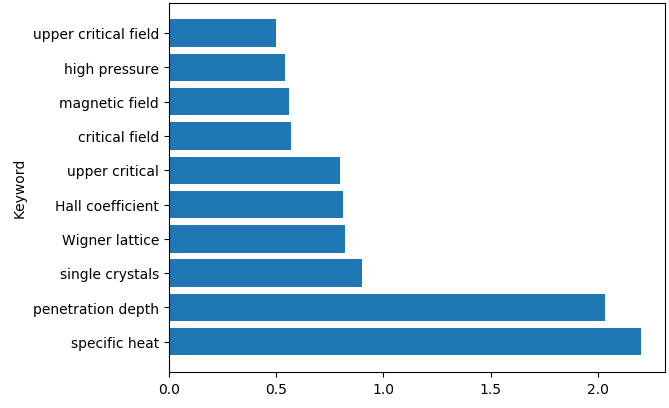
\includegraphics[width=\linewidth]{keyword-top10-body-distribution}
%     \captionof{figure}{Distribution by keyword extracted from the articles body. }
%     \label{fig:keyword-top10-body}
% \end{figure}


\begin{figure}[h]
    \centering
    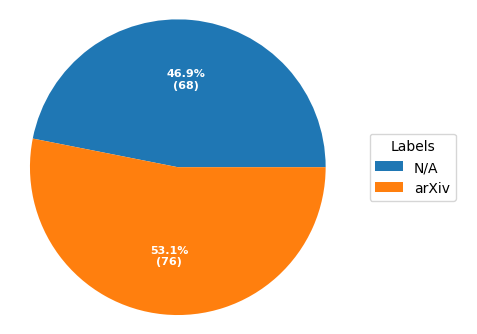
\includegraphics[width=0.7\linewidth]{pie-arxiv-papers.png}
    \captionof{figure}{Rate of arXiv papers.}
    \label{fig:arxiv-rate}
\end{figure}

% Why pdfs? 
The dataset was originated starting from PDFs: 
\begin{enumerate}
    \item The PDF is the most widely used format for scientific publications \cite{johnson2018pdfStatistics}
    % , while other formats, such XML or Latex, are available only on certain platforms
    \item Publishers can provide scientific articles in XML format (with limitations depending on the journal or domain). These versions must be purchased and they are not free to use and redistribute. \item Although the bibliographic data from the publishers comes in higher quality, the body and fulltext might not even be available. 
    \item Despite the effort in following a standardised XML format based on the JATS specification, each publisher uses its own JATS flavour which would require the development of several parser.
    \item Text extracted from PDF represent the "real world" quality of text that can be obtained and could help training a more robust system. [TODO: we need more support for this claim]
\end{enumerate}


\begin{figure}[h]
    \centering
    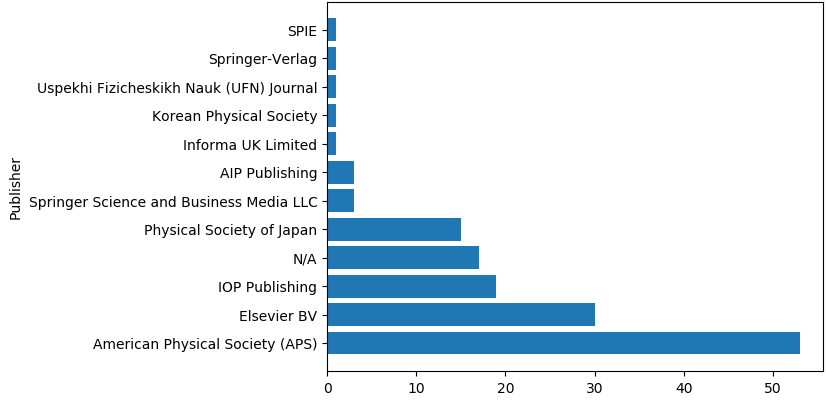
\includegraphics[width=\linewidth]{paper-by-publishers}
    \captionof{figure}{Distribution by publisher automatically extracted from the PDF, and consolidated through lookup to Crossref. }
    \label{fig:distribution-by-publisher}
\end{figure}

\begin{figure}[h]
    \centering
    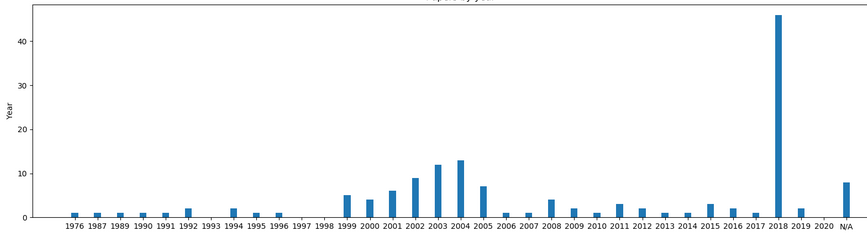
\includegraphics[width=\linewidth]{supermat-distribution-by-year}
    \captionof{figure}{Distribution by publication year, automatically extracted from the PDF, and consolidated through lookup to Crossref. }
    \label{fig:distribution-by-year}
\end{figure}


\subsection{Tag-set design}
The tag-set represents the classes of entities (also called "labels") that are expected to be extracted from the text. 
The tag-set was designed and validated by domain experts and they are summarised and categorised (result, condition, measurement or sample) in Table \ref{table:summary-entities-superconductor}.

\begin{table}[h!]
    \centering
    \begin{tabular}{ | m{6em} | m{4cm} | m{5em} | m{6em} | } 
    \hline
        Name & Description & Type & Label\\ [0.5ex] 
    \hline\hline
        T\textsubscript{c} & Superconducting critical temperature & result & \texttt{<tcValue>}\\ 
    \hline
        T\textsubscript{onset} & Temperature at which the electrical resistance starts to decrease sharply & result& \texttt{<tcValue>}\\
    \hline 
        T\textsubscript{zero} & Temperature at which zero resistance starts to appear & result & \texttt{<tcValue>}\\ 
    \hline
        P & Superconducting applied pressure & condition& \texttt{<pressure>}\\
    \hline
        Material & Material composing the sample & sample & \texttt{<material>}\\
    \hline
        Class & Material classification according to the superconducting domain & sample & \texttt{<class>}\\
    \hline  
        Substrate & Material used to grow sample on it & sample & \texttt{<material>}\\
    \hline
        Crystal structure & Crystal structure, or structure type when adjoined to a material or sample definition & sample & \texttt{<material>}\\
    \hline
        Sample form & Form of the sample: thin film, single crystal, poly crystal, wire, powder & sample & \texttt{<material>}\\
    \hline 
        Fabrication & Indicate the fabrication process of the sample, when adjoined to the sample or material name  & sample & \texttt{<material>}\\
    \hline 
        Measurement method & Method used for measuring the superconducting critical temperature & condition & \texttt{<me\_method>}\\
    \hline
%        H\textsubscript{c1} & Lower Critical field & condition\\ 
%    \hline
%        H\textsubscript{c2} & Higher Critical field & condition\\ 
%    \hline
%        I\textsubscript{c} & Critical current & condition\\
%    \hline
%        J\textsubscript{c} & Critical current density & condition\\ 
%    \hline
%        H\textsubscript{ivr} & Irreversibly field & condition\\
%    \hline    
%        Fabrication process & process used to fabricate the sample & sample\\
%    \hline    
    \end{tabular}
    \caption{Summary of the needed information to be extracted from superconductor research papers}
    \label{table:summary-entities-superconductor}
\end{table}


\textbf{Class} (tag: \texttt{<class>}) represent an arbitrary group of materials by certain characteristics. The definition of class doesn't follow any strict rule but it is learned by domain experts with experience. Classes are organised in a two-level-hierarchy, as illustrated in Figure \ref{fig:class-hierachy}. 

\textbf{Material} (tag: \texttt{<material>}) identifies a name of one or more materials or a sample [TODO: we need a better definition of "sample"]. 
This label is used to collect a various selection of information: 
\begin{itemize}
    \item formula indicate the material as a general or stochiometric formula (e.g. \texttt{LaFe 1-x O7}, \texttt{WB2})
    \item material name indicate the material with the conventional name (e.g. \texttt{YBCO}, \texttt{Metal Diborite}, \texttt{Boride})
    \item shape or form, which indicate the shape the material or sample is created: single crystal, poly crystal, wire, powder, crystal, thin film
    \item doping as expressed as added material (\texttt{Zn-doped}, \texttt{Si-doped}) or percentage of doping (\texttt{2\%-doped}), we consider also general definitions as \textit{overdoped}, \textit{lightly doped}, \textit{pure} as valid information because they can be used by author as quick reference for the sample type in the paper 
    \item fabrication process provides information on how the material has been fabricated. The fabrication process is usually a specific paragraph, this information is only used for discriminating different sample, which were created on a slightly different fabrication process. 
\end{itemize}

\textbf{Superconducting critical temperature expression} (tag: \texttt{<tc>}) is used to identify expressions providing information about the phenomenon of superconductivity which is related to a critical temperature. When a mention of a temperature is found in the text, there is not guaranteed such mention refers to the superconducting critical temperature, it could refer to a general temperature where some event occurs such as the Néel temperature, or the magnetic temperature. This label identify reference to the presence (e.g. \textit{This material is a superconductor}) or absence (e.g. \textit{This material is not a superconductor}) of superconductivity.
In addition, modifiers of these information (superconducting is increasing, decreasing, etc.) are also retained. 

\textbf{Superconducting critical temperature value} (tag: \texttt{<tcValue>}) represent the temperature at which the superconductivity occurs. This includes also boundaries conditions, such as the \textit{onset of superconductivity}, \textit{zero resistance}. 

\textbf{Applied pressure} (tag: \texttt{<pressure>}) indicate the applied pressure when superconductivity occurs. 

\textbf{Measurement method} (tag: \texttt{<me\_method>}) indicates the techniques used to measure or calculate the presence of superconductivity. There are four main classes of methods: theoretical/calculated, electrical resistivity, magnetic susceptibility and specific heat. 
(TODO: add more information why we take only these four type of information]

\begin{figure}[h]
    \centering
    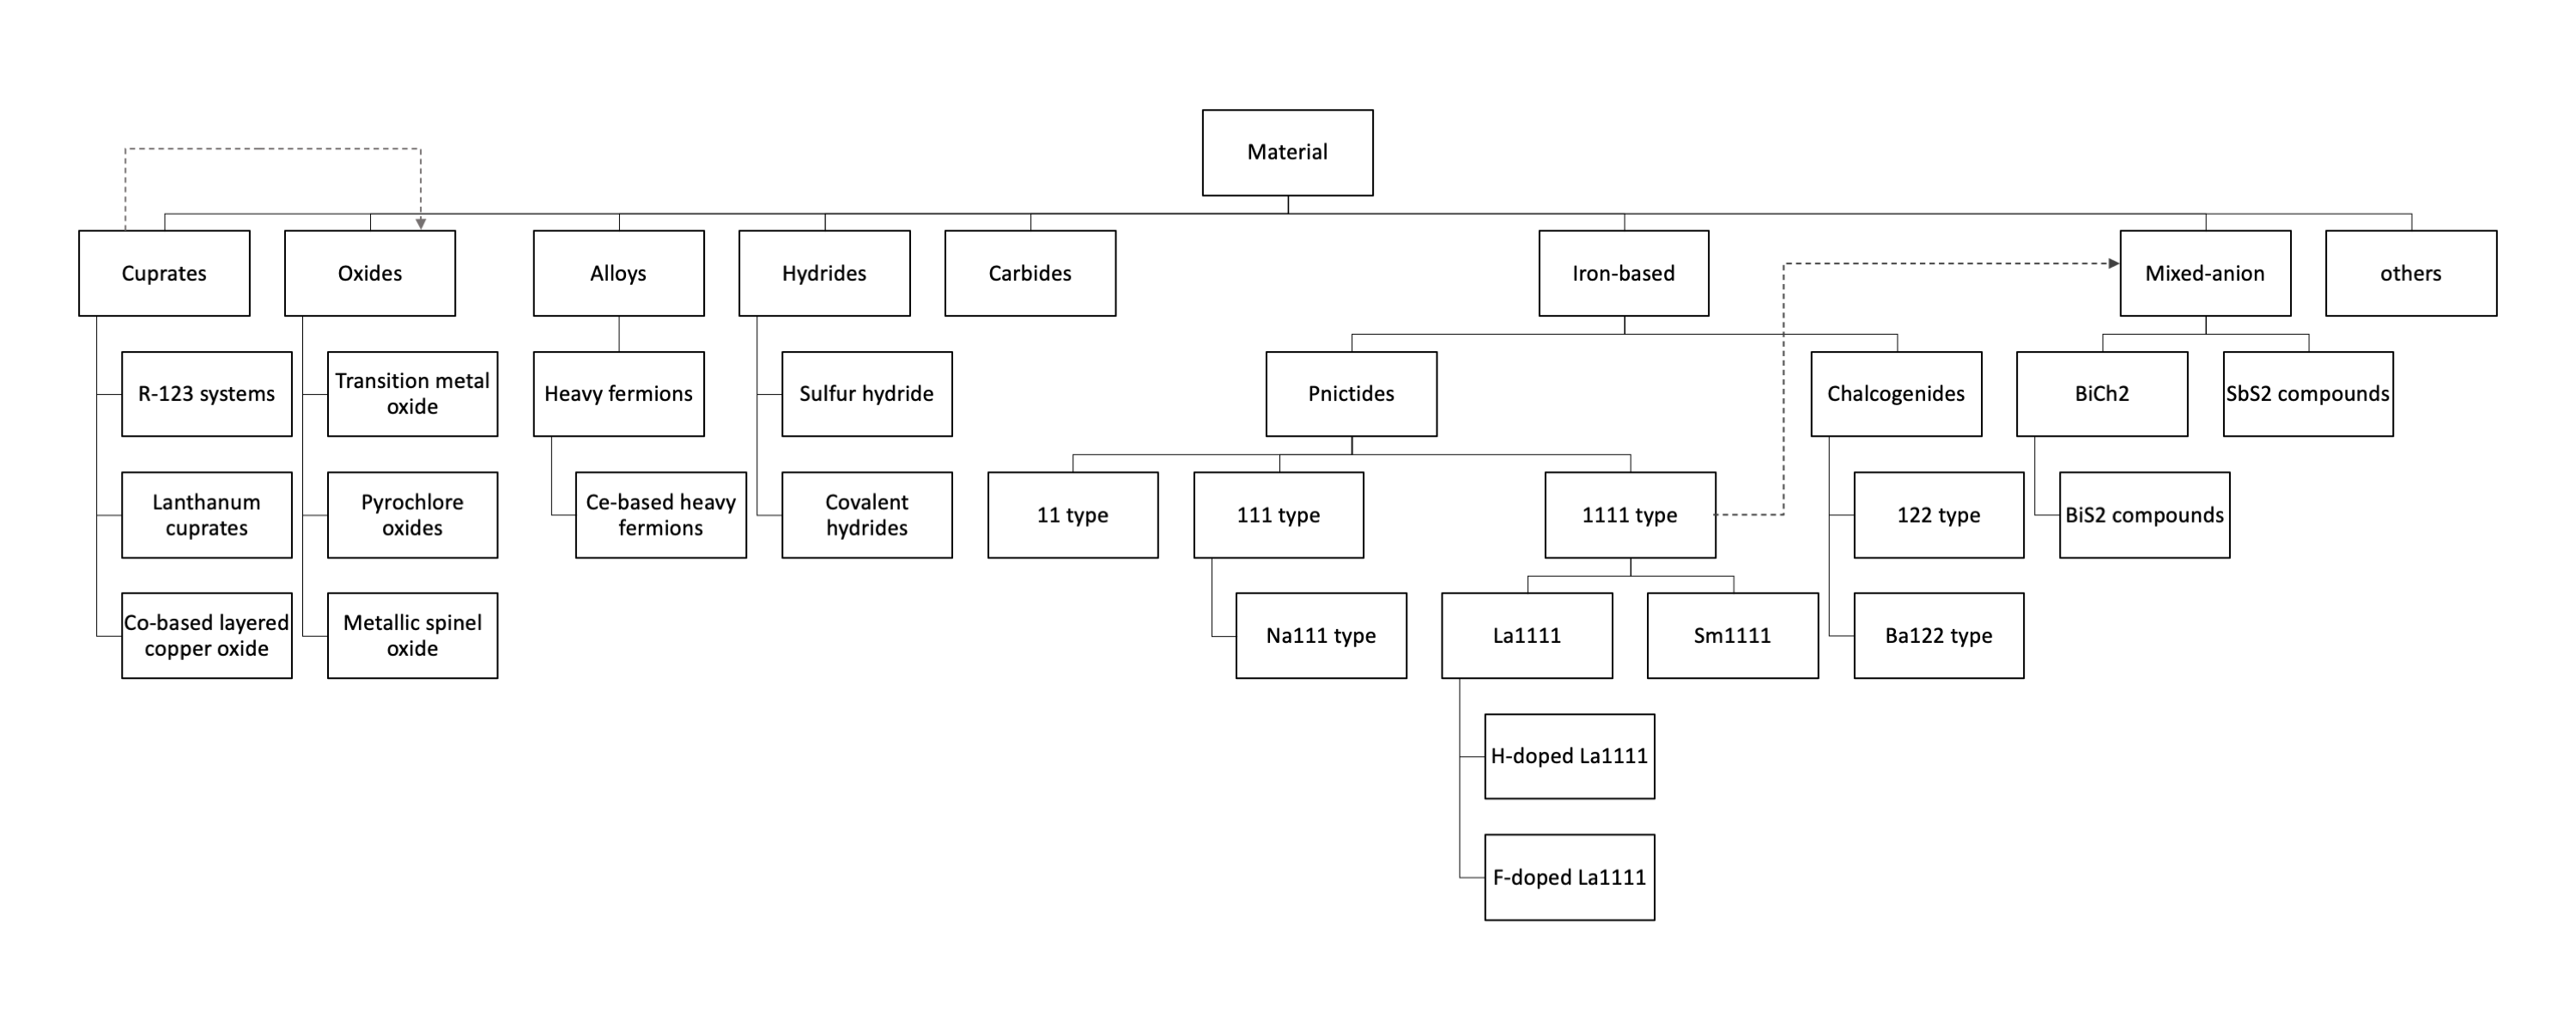
\includegraphics[scale=0.4, angle=90]{classes-superconductors-hierarchy}
    \captionof{figure}{Hierarchy of schema of the superconductors classes. }
    \label{fig:class-hierachy}
\end{figure}

\subsection{Annotation process}
\label{sec:annotation-process}
The annotation process was designed from scratch taking in account previous experiences and related work~\cite{dieb}

Before beginning the work on this dataset, we worked on two main preliminary tasks: a) build an automatic system prototype, and b) perform a preliminary annotation study, which are described in details in sections \ref{subsec:automatic-system-prototype} and \ref{subsec:preliminary-annotation-study}, respectively.

The annotation process was  composed three main components, however we performed two preliminary tasks Before discussing them, we  two preliminary tasks and 

Then, we structured the annotation process into three components: the workflow (Section \ref{subsec:annotation-workflow}, the annotation guidelines (Section \ref{subsec:annotation-guidelines} and the data transformation (Section \ref{subsec:transformation-of-data}. 


\subsubsection{Automatic system prototype}
\label{subsec:automatic-system-prototype}
The prototype of the automatic system~\cite{foppiano2019proposal} allowed us to rapidly assess the feasibility of the project. 
The system was developed as a separate module of an Open Source ML-based library for TDM processes of scholarly publication: Grobid (Generation of Bibliographic Data)~\cite{GROBID}. 
Grobid provides already several basic, yet complex, functionalities: training and evaluation interfaces, access to low-level information from the PDFs (font information, styles, PDF coordinates, etc.), and a REST API. 
This prototype has been built as a domain-specific modules for materials science, which was added to the already existing one: grobid-quantities\cite{foppiano2019quantities} for extracting physical quantities, grobid-astro~\footnote{\url{}} for astronomical object recognition, grobid-dictionaries~\cite{grobid-dictionaries} for structuring dictionaries, to mention few of them. 
Our prototype was extracting materials and their superconducting critical temperature. The process was implemented combining materials names extracted using a newly built \textit{superconductors} model, and the Grobid module for physical quantities (grobid-quantities).
The prototype defined our end to end baseline (described in \cite{foppiano2019proposal}) and implemented other technical features, such as the on-the-fly highlights of pdfs, a REST API. 
The system was modified to accommodate new labels and it was used for pre-annotation, training and evaluation (\textit{Automatic process} in Figure \ref{fig:schema-comparison}).

\subsubsection{Preliminary annotation study}
\label{subsec:preliminary-annotation-study}

We performed a preliminary annotation study to extend the limited training data created for the prototype. This study consists in comparing the annotation of three separate annotators (not domain experts) on the same documents and to record the evolution over several iterations. 
The goals of this study were multi-fold: a) definition of a preliminary tag-set schema, b) knowledge acquisition/improvement, c) measuring and monitoring the agreement over several iterative sessions, and d) discovering caveat and problems as soon as possible. 
The outcome were then discussed and validated with the domain experts. 

% This section should describe how we are doing and which problems we are facing
We selected two OA papers related to superconductivity from the arXiv repository. We defined a reduced tag-set composed by four labels: \texttt{<material>}, \texttt{<tc>}, \texttt{<propertyValue>} and \texttt{<substitution>}. 

\begin{table}[h!]
    \centering
    \begin{tabular}{ | m{10em} | m{20em} | } 
    \hline
        Name & Description \\ [0.5ex] 
    \hline\hline
        \texttt{<material>} & material, sample \\
    \hline
        \texttt{<tc>} & expression describing the presence of absence of superconductivity \\
    \hline
        \texttt{<propertyValue>} & value of properties, in this case it was limited to the superconducting critical temperature \\
    \hline
        \texttt{<substitution>} & substitution values, such as stochiometric values, usually expressed as x or y  \\
    \hline
    \end{tabular}
    \caption{Summary of the preliminary annotations}
    \label{table:summary-preliminary-annotation}
\end{table}

We performed three iterative cycles of annotations, at the end of which, after calculating our Inter Annotation Agreement (IAA) we reviewed the discrepancies. 

In Table \ref{table:summary-iaa} we summarise the IAA in these iterations. We notice that \texttt{<substitution>} was the more unclear label, as had very low agreement until the 3rd iteration. This is due to the fact that it was appearing in many different form. On the other hand any mention of critical temperature (label \texttt{<tc>}) was more clear (reach 85\% agreement at iteration 2). 

\begin{table}[h!]
    \centering
    \begin{tabular}{ | c | c| c| } 
    \hline
        Iteration \# & IAA & IAA by label  \\ [0.5ex] 
    \hline\hline
        1  & 0.45
        &\begin{tabular}{  c | c  } 
            \texttt{<material>} & 0.45\\ 
            \texttt{<tc>} & 0.56\\
            \texttt{<propertyValue>} & 0.50\\
            \texttt{<substitution>} & 0.21\\
        \end{tabular}    
        \\ 
    \hline
        2 & 0.65
        &\begin{tabular}{  c |  c  } 
            \texttt{<material>} & 0.75\\ 
            \texttt{<tc>} & 0.85\\
            \texttt{<propertyValue>} & 0.85\\
            \texttt{<substitution>} & 0.39 \\
        \end{tabular}          
        \\ 
    \hline
        3 & 0.89
        & \begin{tabular}{  c | c  } 
            \texttt{<material>} & 0.89\\ 
            \texttt{<tc>} & 0.91\\
            \texttt{<propertyValue>} & 0.88\\
            \texttt{<substitution>} & 0.94\\
        \end{tabular}       
        
        \\ 
    \hline
    \end{tabular}
    \caption{Summary of the IAA for each of the three cycles of annotation. Together with the average annotation agreement, we publish the agreement by label.}
    \label{table:summary-iaa}
\end{table}

% At the end of this exercise the label \texttt{propertyValue} was renamed \texttt{tcValue} and \texttt{substitution} was merged with \texttt{material}. 

\subsubsection{Transformation of data}
\label{subsec:transformation-of-data}
The PDFs are transformed to text using the Grobid library~\cite{GROBID}, which allow to structure the information in the PDF and recognise the various components, title, author, abstract body, etc. 

During the process information like the reference callout and reference to tables and figures are removed. 
Caption of tables and figures are retained because they might contain material information. 

The output data is an XML file divided by paragraphs. The first paragraph contains the title, the second the abstract, then the body.



\subsubsection{Annotation guidelines}
\label{subsec:annotation-guidelines}
The annotation guidelines describe the principles, and the rules to follow for creating additional data for the SuperMat dataset.
They are divided into four parts. The (a) general principles describe the main rules and convention that are applied in the guidelines. The (b) tag-set provide a detailed description of each label with examples and references. Following, the (c) linking rules are providing all the information related to connect entities that are in a relationship. Finally the (d) out of scope provide a list of elements that are ignored temporarily, or permanently. 

The guidelines were built using a dynamic markup language (ReStructured Text) and stored in a version control system repository such as git\footnote{\url{https://git-scm.com/}}. This allows the latest version to be immediately available after modification as a centralised website, or, converted in multiple formats (pdf, html, epub, etc.) without any additional effort. 

\subsubsection{Annotation workflow}
\label{subsec:annotation-workflow}
The annotation workflow was designed following the schema initially designed by \cite{pustejovsky2012natural}, which defined the iterative process called \textit{MATTER}: Model, Annotate, Train, Test, Evaluate, and Revise.

We have modified this model to better fit in our workflow obtaining five steps: \textit{Pre-annotate}, \textit{Annotation correction}, \textit{Validation}, \textit{Train}, \textit{Test and Evaluate}, \textit{Revise}, as illustrated in Figure \ref{fig:schema-comparison}. 

\begin{figure}[h!]
\centering
\begin{subfigure}{.5\textwidth}
  \centering
  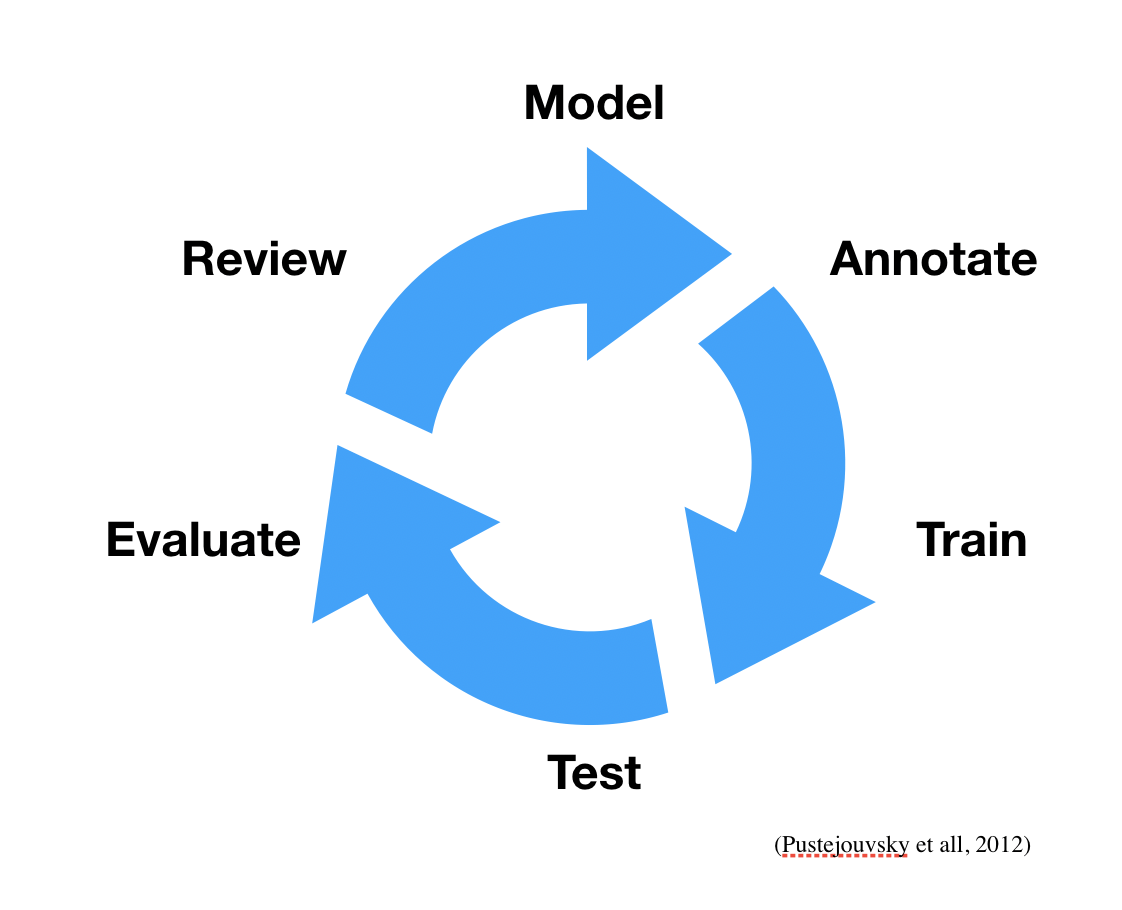
\includegraphics[width=\linewidth]{matter-schema}
  \caption{The \textit{MATTER} schema}
  \label{fig:sub1}
\end{subfigure}%
\begin{subfigure}{.5\textwidth}
  \centering
  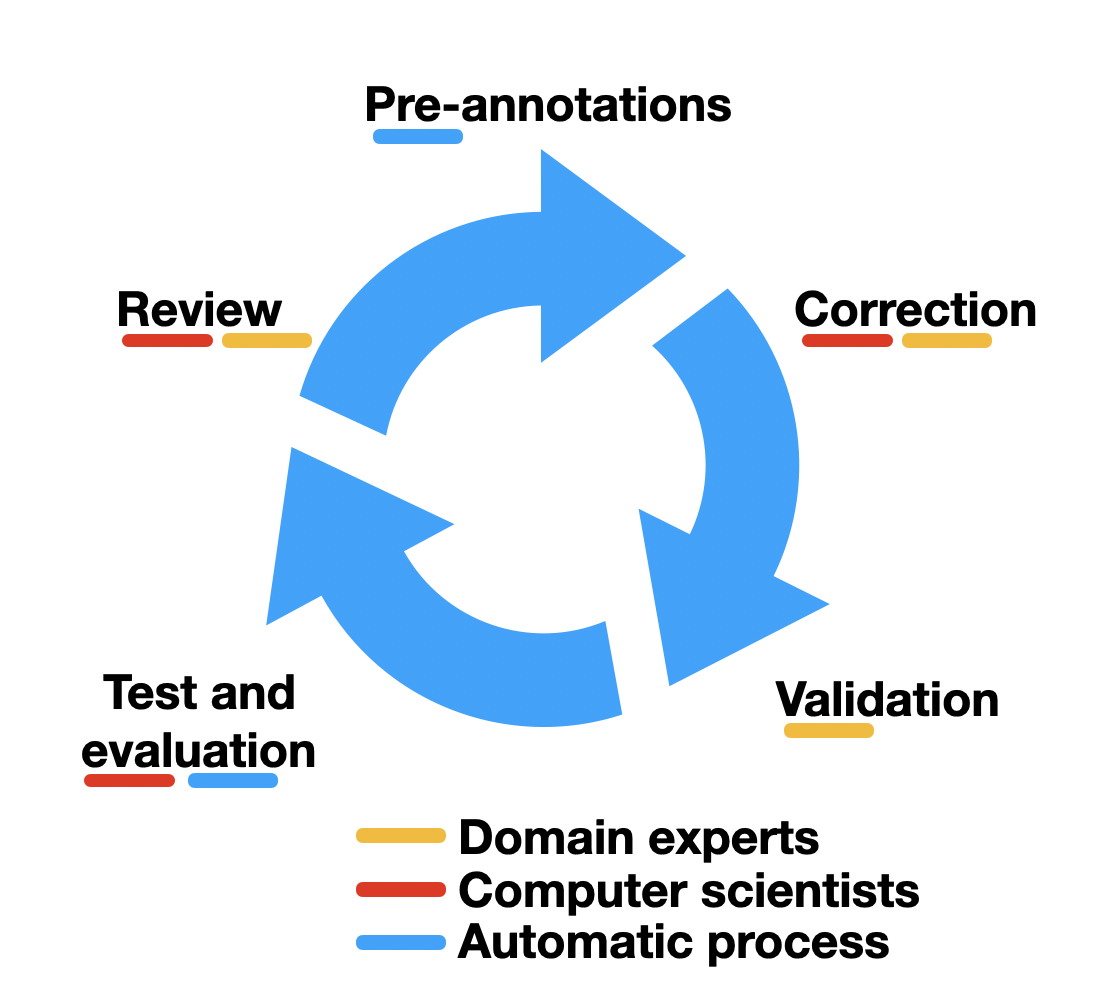
\includegraphics[width=\linewidth]{matter-grobid-schema}
  \caption{The annotation workflow}
  \label{fig:sub2}
\end{subfigure}
\caption{A comparative image of the original \textit{MATTER} schema and the annotation schema we have adopted. }
\label{fig:schema-comparison}
\end{figure}

In our workflow there are three main actors: the automatic system, the computer scientists and the domain experts.

\textbf{Machine-based annotated data / Pre-annotations}
The first step of the annotation process is to generate pre-annotated data from unlabelled documents using the latest implementation available. This is usually the result of the latest trained ML model.  
At the first iteration, since there is no model, this task can be skipped or it can be implemented by a simple rule-based algorithm. In general correcting pre-annotated data is easier than working with plain text. 
If there are several models in cascade, the annotated data will be generated for each models.

\textbf{Annotation correction}
The annotation process, also defined as "correction work" consists of manually correcting the documents and adding/removing or modifying the annotated information, following the annotation guidelines. 
Once a document is completed, is it marked as "Annotated" and can be picked up for Validation, explained in the next subsection. 
%It’s is very important that all mistakes and information are kept up-to-date in the documentation. In such case, the procedure is to open a new issue in the GitLab issues project page and follow the discussion there. Written discussions will facilitate, in future, the understanding of certain decisions.

\textbf{Validation from Domain experts}
The validation is an additional step that ensure a) double verification of the information, b) easily discovering eventual distraction errors, and c) verification and validation from domain experts before. 


\textbf{Review}
Training and evaluation is performed and the results examined. The results (Precision, Recall, F-score) for all the models have been obtained using 10-fold cross-validation (average metrics over the 10 folds).

At the end of each iteration, we review the evaluation improvements or regressions. Plan new changes or a new batch of documents to be corrected in the next iteration. in this phase also the model and the guidelines are reviewed.

\subsubsection{Inter Annotation Agreement}

Analyssi on the inter annotation agreement 


\section{Data Record}
Description of the analysis of the dataset 

This section should be used to explain each data record associated with this work, including the repository where this information is stored, and to provide an overview of the data files and their formats. Each external data record should be cited using our data citation format format.


\section{Applications}
How the corpus can be used

\section{Technical Validation} 
This section should present any experiments or analyses that are needed to support the technical quality of the dataset. This section may be supported by figures and tables, as needed.

Write about the results of the comparison between 
- CS vs DE 
- MS vs DE
- Kubokawa-san / Meng-san vs DE? 

%\section{Data Usage} 
%Describe how the data is provided XML, JSON... 

\section{Code Availability}
where, how the data will be distributed 

Github? MDR, Nomad? 


\section{Conclusion}
Conclusions and future work 

% IAA
% We have analysed the process and the evolution of the agreement during our process and how this can be used to understand when certain constraints or definition are to be clarified further. 
On the creation of annotation we should improve the process of creating training data, especially when the domain expert will be actively involved in task. 

\bibliographystyle{unsrt}
\bibliography{references}  

\end{document}
